% SuperHK - Osc3++ 
% author: Tommaso Boschi
%

\documentclass[a4paper, 11pt]{article}
\usepackage[T1]{fontenc}
\usepackage[utf8]{inputenc}
\usepackage[english]{babel}

\usepackage{xcolor}
\usepackage{listings}	 
\lstset{basicstyle={\footnotesize\ttfamily},
	showstringspaces=false,
	commentstyle=\color{blue},
	keywordstyle=\color{green!80!black},
	stringstyle=\color{red},
}


\usepackage[left=1.00in,right=1.00in, top=1.25in, bottom=1.25in]{geometry}
\usepackage[colorlinks,, urlcolor=blue]{hyperref}

\usepackage{graphicx}
\usepackage{booktabs}

\usepackage{multirow}
\usepackage{multicol}

\usepackage[numbers,sort&compress]{natbib}
\bibliographystyle{inspire}

\usepackage[np]{numprint}
\npthousandsep{\,}
\npdecimalsign{.}
\npproductsign{\times}
\npfourdigitnosep

%maths command
\usepackage{amsmath}
\usepackage{amssymb}
\usepackage{physics}
\usepackage{bbold}
\usepackage{bm}

\newcommand{\ferm}{\mathfrak{f}}
\newcommand{\bs}{\boldsymbol}
\newcommand{\cj}{\overline}
\newcommand{\uj}{\underline}
\newcommand{\pd}{\partial}
\newcommand{\sk}{\hat\varepsilon}

%references
\newcommand{\refeq}[1]{Eq.~(\ref{#1})}
\newcommand{\reffig}[1]{Fig.~\ref{#1}}
\newcommand{\refsec}[1]{Section~\ref{#1}}
\newcommand{\refref}[1]{Ref.~\cite{#1}}

%others
\newcommand{\tapi}{\textsuperscript}
\newcommand{\tped}{\textsubscript}
\mathchardef\mhyphen="2D




\title{\texttt{osc3++}: a combined fitting tool for \\ beam and atmospheric samples}
\author{Tommaso Boschi \\ \href{mailto:tommaso.boschi@kcl.ac.uk}{\small \tt tommaso.boschi@kcl.ac.uk}}



\begin{document}

\maketitle

\fontfamily{lmr}\selectfont


\section{Introduction}
\label{sec:intro}
\texttt{osc3++} was originally developed by R. Wendell and M. Jiang of Kyoto University %
to provide a flexible framework capable of fitting simultaneously beam and atmospheric data %
in view of combined analyses of Super-Kamiokande (SK) and Hyper-Kamiokande (HK).
Since then, the code has gone through various stages of development and structural changes %
to become more modern, portable, and user friendly.
The working principle and the underlying philosophy, however, have not changed.

The \texttt{osc3++} framework is a bundle of computational and plotting utilities helpful to asses the sensitivity %
of a future experiment like HK to neutrino oscillation parameters.
This process is fundamental during the design phase of the experiment and  %
at any stage of the experiment it is important to asses the impact of systematic errors on the total sensitivity.
Even if real data is not available, it is possible to understand whether the planned volume of data to be collected %
has enough constraining power to achieve the target precision.
The oscillation and systematic parameters are input to a Monte Carlo simulation %
to build the expected distribution of events.
This expected data is then compared to simulated ``observed data'', which is created by selecting %
a preferred combination of oscillation parameters in order to mimic the real distributions of events %
that will be eventually collected.
Scanning over the oscillation parameters, the resolution to oscillation parameters and, more importantly, %
the influence of the systematic uncertainties can be studied.

The workflow of the framework can be structured as follows
\begin{itemize}
	\item a combination of oscillation parameters is chosen to be the ``true'' (observed) one;
	\item beam and atmospheric predictions at the detector are built twice, using the ``true'' %
		combination of parameters (observed events) and using a combination under examination (expected events);
	\item a $\chi^2$ between observed and expected events is created as a function of the systematic parameters;
	\item the minimum value of $\chi^2$ is found with respect to the systematic parameters;
	\item the process is repeated at different combinations of oscillation parameters.
\end{itemize}

In this document, the main modules of the software are explained in detail.


\section{Getting started}

The framework can be found on \href{https://github.com/tboschi/SuperHK}{GitHub}.
Simply run
\begin{lstlisting}[language=bash]
	git clone https://github.com/tboschi/SuperHK.git
\end{lstlisting}
to clone the latest version of the repository.
The framework is a bundle of bash scripts and C++ code.
The executables should not be run on their own, but always through the scripts %
because the script utilities are used to perform additional checks on the folder structure, %
change configuration files, or submit jobs to the cluster.

\subsection{Requirements}

The requirements for the code to be compiled and run are
\begin{itemize}
		\small
	\item \textbf{make};
	\item \textbf{gcc-c++} version 4.8 or higher (for C++11);
	\item \textbf{ROOT} version 5.34/38 or higher;
	\item \textbf{Eigen} version 3.3 or higher;
	\item \textbf{HTCondor} or \textbf{Slurm} as workload managers, for distributed computing.
\end{itemize}

Before starting compilation, the \href{https://root.cern.ch/}{ROOT data analysis framework} %
should be installed and properly linked.
A simple test to check that is to run
\begin{lstlisting}[language=bash]
	root-config --glibs --cflags
\end{lstlisting}
If the output looks reasonable, then ROOT is correctly installed.
Please refer to their documentation on how to install the framework.

Another library necessary is the \href{http://eigen.tuxfamily.org/}{Eigen library}.
It does not need to be compiled as it is an only header library.
If Eigen is already installed in the user system, it is necessary to define the environment variable \texttt{EIGEN} %
pointing to the installation location.
\begin{lstlisting}[language=bash]
	export EIGEN=/path/to/eigen
\end{lstlisting}
It is important to note that this is the path to the top folder containing the actual headers, %
usually under a folder called \texttt{Eigen} (note capitalisation).
Another option is to simply copy the full folder \texttt{Eigen} to the local \texttt{include} folder.

Certain executables perform better when distributed on a computing cluster.
The scripts only support either HTCondor or Slurm as workload managers.
It is assumed that the file system is shared by each node on the cluster.
If that is not the case, as for a universe grid system, then some scripts may not work out of the box.

\subsection{Compiling}

Compilation on the local machine is done with
\begin{lstlisting}[language=bash]
	make
\end{lstlisting}
If only one binary is needed, this can be specified with
\begin{lstlisting}[language=bash]
	make APP=<main>
\end{lstlisting}
where \texttt{main} is any main file under the local \texttt{app} folder.
The \texttt{.cpp} extension must be omitted.
For example, to compile just the fitter executable, it is possible to run
\begin{lstlisting}[language=bash]
	make APP=fitter
\end{lstlisting}
as there is a main function in the file \texttt{app/fitter.cpp}.

\subsection{Cross-compilation}

Due to the default flags passed to the gcc compiler (\texttt{-O3 -march}), the executables are highly optimised %
for the native architecture.
The flags are needed to activate special vector instructions required by Eigen which speed up %
the computation quite considerably.
The disadvantage of those flags is that the binaries can only run on the local architecture or compatible ones.
This can be problematic when running parallel jobs on a distributed cluster as different architectures %
not compatible with each other might be present.

This problem can be overcome by compiling the code on each node of the cluster.
An utility to do this is available and it is simply run as
\begin{lstlisting}[language=bash]
	./cross-compile.sh
\end{lstlisting}
It is not cross-compilation properly speaking, as both scripts first determine the nodes %
on the cluster, then ssh into each node and only if a new architecture is found a new, optimised binary is compiled %
for that particular architecture.
This workaround works as long as access to the file system is shared on the cluster and that each node can %
be accessed via ssh by the user.

The user can test if they can ssh into a node of the cluster first.
If this is not possible, then the \texttt{cross-compile.sh} script will not work.
The user should manually edit the \texttt{Makefile} and remove the \texttt{-march=native} flag and %
compile locally with \texttt{make}.

\subsection{Setting up the environment}

After a successful compilation, the environment is set up with the utility
\begin{lstlisting}[language=bash]
	./setup.sh
\end{lstlisting}
This builds the folder structure required by the framework and downloads the input files from %
\url{http://hep.lancs.ac.uk/~tdealtry/oa/} and \url{https://pprc.qmul.ac.uk/~tboschi/HK/atmo}.
The result directory can be specified with the \texttt{-p <prefix>} option.
By default, the prefix is a new folder called \texttt{errorstudy} inside the current working directory.
The subfolders
\begin{itemize}
		\small
	\item \texttt{<prefix>/reconstruction\_beam} and
	\item \texttt{<prefix>/reconstruction\_atmo}
\end{itemize}
are created to contain reconstruction files to build the beam and atmospheric data samples.

Now the framework is ready for analysis.
In the following examples, it will be assumed that the result directory is the default one, %
\texttt{errorstudy}.

\subsection{Running the fitter}

The fitter is the most important tool of the framework, %
whereas the other executables are used for validation or plotting.
Before running it, the user has to decide which sample to fit:
\begin{itemize}
	\item the beam sample;
	\item the atmospheric sample;
	\item the beam and atmospheric samples together.
\end{itemize}
Next, the true and fitted neutrino mass hierarchy should be chosen and whether or not %
fit the systematic errors.
The systematic files should be provided in any case.

A new folder in the analysis directory should be created whenever the samples or the systematic models are changed.
For example,
\begin{lstlisting}[language=bash]
	mkdir errorstudy/first_run
\end{lstlisting}
Then, a sub folder containing the systematic files should be created (or copied) in this new directory.
The nominal T2K 2018 systematic model is found under \texttt{errorstudy/0}, therefore
\begin{lstlisting}[language=bash]
	cp -r errorstudy/0/systematics errorstudy/first_run
\end{lstlisting}

Finally, the fitter can be launched on the distributed computing system with %
the \texttt{trisens.sh} utility.
For example,
\begin{lstlisting}[language=bash]
	./trisens.sh -r errorstudy/first_run -d comb -1 NH -2 NH -N 500
\end{lstlisting}
will launch 500 jobs (\texttt{-N 500}) on the cluster, fitting both the beam and atmospheric samples %
(\texttt{-d comb}) with true and fitted normal mass hierarchies (\texttt{-1 NH -2 NH}).
Other important options are 
\begin{itemize}
		\small
	\item \texttt{-s} to do a statistics only fit, i.e.\ no systematics;
	\item \texttt{-f <scan\_type>} to perform a scan fit, i.e.\ changing the true point at each iteration %
		as it is done for CPV sensitivity studies;
	\item \texttt{-v <verbosity>} to change the verbosity of the log files.
\end{itemize}
The full list of options can be shown with
\begin{lstlisting}[language=bash]
	./trisens.sh -h
\end{lstlisting}
The utilities automatically edit the card files in the \texttt{cards} folder and place copies %
in the folder
\begin{lstlisting}[language=bash]
	errorstudy/first_run/NH_NH/sensitivity/
\end{lstlisting}
An \texttt{.info} file will be created as well with a name determined by the scan type.
A single fit creates a \texttt{point.info} file containing the number of the point fitted, %
whereas a fit scan for CPV creates a \texttt{CPV\_scan.info} file with a list of all the %
points fitted.
Once the fitter is finished the output results will be stored in the folder %
\begin{lstlisting}[language=bash]
	errorstudy/first_run/NH_NH/sensitivity/point_<p>
\end{lstlisting}
where \texttt{<p>} is the point in the oscillation space. For example, \np{49773} is the nominal (\emph{true}) %
fit point of the default oscillation parameter space, defined in \texttt{cards/oscillation.card}.
In the output folder, there will be
\begin{itemize}
		\small
	\item 1 submission file, with name \texttt{R....sub};
	\item 1 card file called \texttt{this\_sensitivity.card} which links other cards in the above directory;
	\item $N_\text{jobs}$ ROOT files, with names starting with \texttt{SpaghettiSens...};
	\item $N_\text{jobs}$ log files, with names \texttt{L....log};
\end{itemize}
where $N_\text{jobs}$ is the number of jobs launched.
High level of verbosity will create bigger log files, so the user must pay attention to their disk quota.
Those files are needed for debugging and status purposes only, %
hence if no problem occurred they can be eventually deleted (see below).
The output ROOT files also take up a lot of space, but they contain the actual results, stored under \texttt{TTree} objects called \texttt{stepX2Tree}.
%The entries of the \texttt{TTree} objects will have around
%\[
	%\frac{\text{number of points}}{500}\ \text{entries}
%\]
%where the number of points of the default space is \np{195871}.

\subsection{Checking the jobs}

The user should use their manager queue utility to control the status of their jobs.
This command is
\begin{lstlisting}[language=bash]
	condor_q -sub $USER  # for HTCondor
	squeue -u $USER      # for SLURM
\end{lstlisting}
Once the jobs are done, it is wirth checking whether they were successfull, %
as it may happen that some job fails.
This could be due to many reasons, e.g.\ job request rejected by the manager.
As a full fit requires many resources and can take a long time to complete, %
an utility to fix broken or missing jobs it is provided.
Using the previous example, this is done with
\begin{lstlisting}[]
	./complete.sh errorstudy/first_run/NH_NH/sensitivity/CPV_scan.info
\end{lstlisting}
The script reads through the log files checking whether the respective job completed.
If not, that specific job is relaunched.
The script detects also if a whole point is skipped by any reason and can resubmit the full job for that point.
If no error message is displayed, then the fitter concluded successfully and the log files may be deleted.

\subsection{Extracting the results}

The $\chi^2$ contours can only be created for single fits (not scans) by calling
\begin{lstlisting}[language=bash]
	./contours.sh errorstudy/first_run/NH_NH/sensitivity/point_<p>
\end{lstlisting}
and the result is saved in 
\begin{lstlisting}[language=bash]
	errorstudy/first_run/NH_NH/contours/point_<p>.root
\end{lstlisting}
The resulting file contains a list of \texttt{TH1} and \texttt{TH2} objects with the %
$\chi^2$ profile against one or two oscillation parameters.
The processing is done by the \texttt{build\_contours} binary.

CPV sensitivity curves are instead created with
\begin{lstlisting}[language=bash]
	./exclude.sh errorstudy/first_run/NH_NH/sensitivity/CPV_scan.info
\end{lstlisting}
In this case, the \texttt{.info} file which lists all the points scanned over should be passed.
The utility runs the \texttt{exclusion} binary which creates a text file with exclusion power %
at each value of $\delta_\text{CP}$.
The file is saved as
\begin{lstlisting}[language=bash]
	errorstudy/first_run/NH_NH/contours/CVP_scan.dat
\end{lstlisting}

\subsection{Plotting the results}

There are a few plotting utilities that automatically read the result files %
and produce plots and PDF presentations.
These scripts require
\begin{itemize}
		\small
	\item \textbf{gnuplot} version 4.4 or higher with cairolatex terminal;
	\item \textbf{texlive} for pdflatex with beamer;
\end{itemize}
and they are
\begin{lstlisting}[language=bash]
	./plot_contours.sh
	./plot_exclusion.sh
\end{lstlisting}
The scripts create plots that combine results from different fitter runs and it is particularly useful %
when a comparison between systematic models or mass hierarchies is needed.
However, it is important that all the fitter results are from the same oscillation parameter space.
The scripts will detect if that is not the case and will exit.

Before executing them, the user should modify the first lines of each script which will look like this
\begin{lstlisting}[language=bash]
	# output name unique to combination of sets
	name="one_two_three"

	# list of files with CPV scan results
	model=("errorstudy/one/NH_NH/contours/point_xxx.root"
	       "errorstudy/two/NH_NH/contours/point_yyy.root"
	       "errorstudy/three/NH_NH/contours/point_zzz.root")

	# names for displaying above results
	nickn=("one_cpv"
	       "two_cpv"
	       "three_cpv")
\end{lstlisting}
The first variable \texttt{name} is a unique name that identifies the particular combination of results.
The second variable \texttt{model} is the list of input files, whereas the third variable \texttt{nickn} %
is a list of names associated to the input files.
These will be used for labelling the results in the plots.
The scripts will automatically create \LaTeX\ files with all the $\chi^2$ contours. 


\section{Tools module}

This module contains a configuration file parser, done by the \texttt{CardDealer} class.
Given the large number of input parameters needed in the analysis, it is advised to use this class as much as possible.
A configuration file, or \emph{card}, looks like this
\begin{lstlisting}[language=bash]
	# --- /path/to/card ---
	#
	# this is a comment. each line should be in the format
	# key <space> value [, value1, ...]

	float_value	123.321	  # another comment
	integer		-54321
	boolean		0	  # or any other integer
	string		"hello"
	array		1, 2, 3	  # of any type
	key_1		"x1", "y1", "z1"
	key_2		"x2", "y2", "z2"
	key_3		"x3", "y3", "z3"
	...
\end{lstlisting}

A \texttt{CardDealer} object is initialised by passing as argument the name of the configuration file.
Depending on the application, the user can decide to create the object automatically or dynamically.
The constructor is
\begin{lstlisting}[language=C++]
	template <typename T>
	CardDealer(T cardFile, bool verb = false);
\end{lstlisting}
where \texttt{cardFile} is the absolute or relative path to the configuration file and %
\texttt{verb} activates debugging messages.
The file is automatically parsed and a map of key--value(s) is created.
To retrieve a value by its key the templated method \texttt{CardDealer::Get} is available.
There are many implementation of the same function, depending on the signature
\begin{lstlisting}[language=C++]
(1) template <typename T,
    typename std::enable_if<std::is_fundamental<T>::value>::type* = nullptr>
    bool Get(const std::string &key, T &ret);

(2) template <typename C,
    typename std::enable_if<is_sequence<C>::value>::type* = nullptr>
    bool Get(const std::string &key, C &ret);
\end{lstlisting}

\begin{lstlisting}[language=C++]
(3) template <typename T>
    bool Get(const std::string &key, std::map<std::string, T> &ret);

(4) bool Get(const std::string &key, std::string &ret);

(5) bool Get(const std::string &key, std::vector<std::string> &ret);

(6) bool Get(const std::string &key);
\end{lstlisting}
The function always \texttt{true} if the key exists and retrieval was successful, \texttt{false} otherwise.
The actual value associated to the key is returned by reference.
The last implementation (\texttt{6}) only checks if the key exists.
The key must be a \texttt{std::string}, but the value can be of any fundamental type compatible with the literals of the configuration file (\texttt{1}).
If value is array-like, then STL containers with an \texttt{insert} method are supported (\texttt{2}); %
at the moment they are \texttt{std::vector},  \texttt{std::set},  \texttt{std::list},  and \texttt{std::deque}. 
These are selected with the built-in structure \texttt{is\_sequence}.
When multiple keys have the same prefix, they can retrieved collectively into a map (\texttt{3}); the prefix is removed.
It is important that the respective values can be converted to the same type.
In the example above, keys \texttt{key\_1}, \texttt{key\_2}, \texttt{key\_3} have all similar value types (array of strings).
Because of the internal implementation, string values have explicit signatures (\texttt{4}, \texttt{5}).
The best usage for this function is as the following example:
\begin{lstlisting}[language=C++]
	CardDealer cd("/path/to/card");

	double float_value; // create variable
	if (!cd.Get("float_value", float_value))
		float_value = 999.999;	// default value if key does not exist

	// retrieve an array-like parameter
	std::vector<int> array;
	cd.Get("array", array);

	// retrieve a group of parameters
	std::map<std::string, std::vector<std::string> > keys;
	cd.Get("key_", keys);

	for (const auto &ik : keys)
		std::cout << ik.first << "\t" << ik.second.front() << std::endl;
	// output is
	// 1	x1
	// 2	x2
	// 3	x3
\end{lstlisting}

The full list of keys is retrieved with the method
\begin{lstlisting}[language=C++]
    std::vector<std::string> ListKeys();
\end{lstlisting}
The keys must be unique in the card file, otherwise only the last key is considered.
Finally, the following method returns the name of the card
\begin{lstlisting}[language=C++]
    std::string CardName();
\end{lstlisting}


\subsection{Physics module}
\label{sec:physics}

The physics module has the main purpose of calculating the oscillation probability and setting up the oscillation parameter space.
It is divided into three subclasses: the oscillator class, the atmosphere class, and the parameter space class.
There are also two other utilities: the flavour static structure (see below) %
and a physics constant namespace \texttt{Const} defined in \texttt{physics/Const.h}.

\subsubsection{Oscillator class}
\label{sec:oscillator}

The oscillator class is a C++11 implementation of the solution to the three-neutrino flavour picture proposed by Barger and collaborators~\cite{Barger:1980tf}.
The transition amplitude including matter effects is written in the form
\begin{equation}
	A(\nu_\alpha \to \nu_\beta) = \sum_{ij} U_{\alpha i} X_{ij} U_{j \beta}^\dagger\ ,
\end{equation}
where $U$ is the mixing matrix, and it is such that the oscillation probability is
\begin{equation}
	P(\nu_\alpha \to \nu_\beta) = |A(\nu_\alpha \to \nu_\beta)|^2  \ .
\end{equation}
The matrix $X$ satisfies the equation
\begin{equation}
	i \dv{X}{t} = X\,H\ ,
\end{equation}
with $H$ the Hamiltonian, and it as an exact solution for constant matter density $N_e$
\begin{equation}
	X = \sum_k \qty[\prod_{j\neq k} \frac{(2E\,H - M^2_j \mathbb{1})}{\delta M_{kj}^2}] \exp\qty(-i \frac{M_k^2 L}{2E})\ ,
\end{equation}
where $\delta M^2_{ij} = M^2_i - M^2_j$.
The masses $M_i$ are the effective neutrino masses in matter which for the three-neutrino case and constant density %
they read
\begin{equation}
	M^2_i = -\frac{2}{3}(\alpha^2 - 3\beta)^\frac{1}{2} \cos \qty[\frac{1}{3} \acos %
			\qty(\frac{2\alpha^3 - 9\alpha \beta + 27\gamma}{2(\alpha^2 - 3\beta)^{\frac{3}{2}}})] %
			+ m_1^2 - \frac{\alpha}{3}
\end{equation}
with
\begin{align}
	\alpha &= 2\sqrt{2}\,E\,G\,N_e + \delta m^2_{12} + \delta m^2_{13}\ , \\
	\beta  &= \delta m^2_{12} \delta^2_{13} + 2\sqrt{2}\,E\,G\,N_e \,\qty[\delta m^2_{12} (1-|U_{e2}|^2) + \delta m^2_{13}(1-|U_{e3}|^2)]\ , \\
	\alpha &= 2\sqrt{2}\,EGN_e \,\delta m^2_{12} \delta m^2_{13} |U_{e1}|^2\ .
\end{align}

The oscillation amplitude of a neutrino crossing a more complicated matter profile is simply
\begin{equation}
	A(\nu_\alpha \to \nu_\beta) = \sum_{ij} U_{\alpha i} \prod_n X^{(n)}_{ij} U_{j \beta}^\dagger\ ,
\end{equation}
where the matter profile is divided into consecutive slabs of constant density $N^{(n)}_e$ and the matrix $X^(n)$ is computed for %
each length $L^{(n)}$ crossed.

This calculation is done by the \texttt{Oscillator} class in a matricial way. 
To save computational time, the oscillation probability is computed for both neutrino and antineutrinos %
by promoting the $X$ matrices to be $6\times 6$ matrices, as well as the PMNS matrix, %
where the top left $3\times 3$ block corresponds to the neutrino component and the bottom right $3\times 3$ block to the antineutrino component.
The use of an object class requires setting up the matter profile which is represented by an \texttt{Oscillator::Profile}
\begin{lstlisting}[language=C++]
    typedef std::vector<std::tuple<double, double, double> > Profile;
\end{lstlisting}
The three elements of the tuple are length, matter density, and electron yield (the percentage of electrons in matter).
The density profile is created by the constructors.
There are different constructors available and they only differ in how the input parameters are passed.
\begin{lstlisting}[language=C++]
(1) Oscillator(const std::vector<double> &lengths,
	       const std::vector<double> &densities,
	       bool lut = false, double threshold = 1e-9);

(2) Oscillator(const std::vector<double> &lengths,
	       const std::vector<double> &densities,
	       const std::vector<double> &electrons,
	       bool lut = false, double threshold = 1e-9);

(3) Oscillator(const std::string &densityFile,
	       bool lut, double threshold);

(4) Oscillator(const std::string &densityFile;

(5) Oscillator(CardDealer *cd);
\end{lstlisting}
If the electron yield is not given or not known (\texttt{1}), the missing values are filled with 50\%.
For both constructors (\texttt{1}) and (\texttt{2}), the \texttt{Oscillator::Profile} object is created using the input vectors.
The constructor (\texttt{3}) reads the matter profile from the file \texttt{densityFile} by calling the \texttt{GetMatterProfile} static method.
The density file should contain two or three columns with lengths, density, and electron yield if known.
The constructor (\texttt{4}) expects a card file name and build a local \texttt{CardDealer} object, %
whereas constructor (\texttt{5}) accepts an already existing \texttt{CardDealer} object.
These constructors will retrieve a density file defined in the card file as
\begin{lstlisting}[language=bash]
    density_file   "/path/to/density_file"
\end{lstlisting}
The matter profile can be changed at any time with the \texttt{Oscillator::SetMatterProfile} method.

Since oscillation analysis requires the calculation of the same baseline with same energies multiple times and the matter profile is fixed, %
the transition matrices can be stored by setting \texttt{lut} to true in the constructor.
This can save some precious resources only when exactly the same densities and energies are used over and over again, %
as for example for beam oscillation, otherwise no benefit is obtained.
The \texttt{threshold} value refers to the resolution in energy for storing the transition matrix.
These settings can also be changed via card file as
\begin{lstlisting}[language=bash]
    LUT        0 # or 1 to turn on
    threshold  1e-9
\end{lstlisting}

On top of the matter profile, also the mixing parameters and neutrino masses must be specified. For those, the templated methods %
\begin{lstlisting}[language=C++]
    template<pmns type>
    void SetPMNS(double s12, double s13, double s23, double cp);
\end{lstlisting}
where \texttt{mode} can be
\begin{itemize}
		\small
	\item \texttt{pmns::sin} and the arguments expected are in order $\sin \theta_{12}$, $\sin \theta_{13}$, $\sin \theta_{23}$, %
		and $\delta_\text{CP}$;
	\item \texttt{pmns::sin2} and the arguments expected are in order $\sin^2\theta_{12}$, $\sin^2\theta_{13}$, $\sin^2\theta_{23}$, %
		and $\delta_\text{CP}$;
	\item \texttt{pmns::angles} and the arguments expected are in order $\theta_{12}$, $\theta_{13}$, $\theta_{23}$, %
		and $\delta_\text{CP}$;
\end{itemize}
\begin{lstlisting}[language=C++]
    template<masses type>
    void SetMasses(double m1, double m2);
\end{lstlisting}
where \texttt{mode} can be
\begin{itemize}
		\small
	\item \texttt{masses::normal} and the arguments expected are in order $\Delta m_{21}^2$ and $|\Delta m_{32}^2|$;
	\item \texttt{masses::inverted} and the arguments expected are in order $\Delta m_{21}^2$ and $|\Delta m_{32}^2|$;
	\item \texttt{masses::absolute} and the arguments expected are in order $m_2^2$, $m_3^2$, where it is assumed that $m_1^2 = 0$;
\end{itemize}
are available.

The oscillation probability between neutrino flavours is computed, or retrieved if using the LUT, with the method
\begin{lstlisting}[language=C++]
    double Probability(Nu::Flavour in, Nu::Flavour out,
		       double energy, bool force = false);
\end{lstlisting}
which expects as input arguments the neutrino flavours and the particle energy.
The neutrino flavours are specified using the static structure \texttt{Nu} contained in the \texttt{physics/Flavours.h} header.
Some methods are defined in this structure to convert the flavour type to and from PDG particle codes or simply strings,
such as
\begin{lstlisting}[language=C++]
    static Flavour fromString(const std::string &flv);
    static Flavour fromPDG(int pdg);
    static std::string toString(int pdg);
    static std::string toString(Flavour flv);
\end{lstlisting}
The following values are accepted to specify neutrino flavours
\begin{itemize}
		\small
	\item $\nu_e$         can be \texttt{Nu::E\_}, \texttt{Nu::electron}, 12, or \texttt{"nuE0"}
	\item $\nu_\mu$       can be \texttt{Nu::M\_}, \texttt{Nu::muon}, 14, or \texttt{"nuM0"}
	\item $\nu_\tau$      can be \texttt{Nu::T\_}, \texttt{Nu::tau}, 16, or \texttt{"nuT0"}
	\item $\cj{\nu}_e$    can be \texttt{Nu::Eb}, \texttt{Nu::antielectron}, -12, or \texttt{"nuEb"}
	\item $\cj{\nu}_\mu$  can be \texttt{Nu::Mb}, \texttt{Nu::antimuon}, -14, or \texttt{"nuMb"}
	\item $\cj{\nu}_\tau$ can be \texttt{Nu::Tb}, \texttt{Nu::antitau}, -16, or \texttt{"nuTb"}
\end{itemize}
The right utility should be used to convert the flavour type into a \texttt{Nu} object.


\subsubsection{Parameter space class}
\label{sec:paramater_space}

The oscillation parameters are fixed parameters in the analysis, i.e.\ they are not allowed to vary when minimising the $\chi^2$.
These parameters are instead changed at each iteration step, selecting the predetermined combinations on a fixed grid in %
a multidimensional space.
The parameters space class is a tool helpful when working with distributed resources as it allows to linearise this multidimensional %
parameter space and each iteration can be more easily divided among multiple processes.
The parameter space itself is a hyper-grid in the space
\begin{equation}
	\Delta m^2_{21} \times \Delta m^2_{32} \times \sin^2\theta_{12} \times \sin^2 \theta_{13} \times \sin^2 \theta_{23} \times \delta_\text{CP}
\end{equation}
which can be defined by configuration file in the constructor.
In the same configuration file it is possible to determine the nominal --- or \emph{true} --- value of the space %
which equals to the expected combination of oscillation parameters.
The space of each parameter $p$ is linearly divided in $N-1$ segments in the specified range $[p_0, p_N]$ %
so as to have $N$ equidistant points $p_0, p_1, \ldots, p_{N-1}, p_{N}$ and 
\begin{equation}
	p_{i+1} - p_{i} = \frac{p_{N} - p_0}{N-1}\ .
\end{equation}
The card file for the oscillation parameter space has the following format
\begin{lstlisting}[language=bash]

# parm_VAR	low_end		high_end	points	nominal_point

# example for Asimov A space
parm_M12	0.0000753,	0.0000753,	1	
parm_S12	0.307,		0.307,		1	
parm_M23	0.002464,	0.002554,	13,	6
parm_S13	0.0197,		0.0239,		13,	6
parm_S23	0.426,		0.579,		19,	12
parm_CP		-3.14159265359,	3.14159265359,	61,	15

penalty_S13	0.0218, 0.0007
\end{lstlisting}
where the low end corresponds to $p_0$ and the high end to $p_N$.
If the nominal point is not provided, this is assigned by default to be the central point of the interval.
The class also computed Gaussian penalty terms which can be specified for any parameter giving the central and the error value %
of another experimental constrain, ${\vartheta} \pm \sigma_{{\vartheta}}$.
The following $\chi^2$ term is therefore added to the full likelihood
\begin{equation}
	\chi^2_\text{pen} = \frac{(\theta - {\vartheta})^2}{\sigma_{{\vartheta}}^2}
\end{equation}

The number of points in the grid is $\prod_k N^{(k)}$ where $k$ runs over the oscillation parameters.
These points are numbered progressively incrementing the variables in reversed alphabetical order, because %
the variables are stored in maps as strings:
\begin{itemize}
	\item $\Delta m^2_{21}$ and $\Delta m^2_{32}$ are respectively \texttt{M12} and \texttt{M12};
	\item $\sin^2\theta_{12}$, $\sin^2 \theta_{13}$, $\sin^2 \theta_{23}$ are respectively \texttt{S12}, \texttt{S13}, %
		and \texttt{S23};
	\item $\delta_\text{CP}$ is \texttt{CP}\footnote{In future versions of \texttt{osc3++}, this will become \texttt{dCP}.}.
\end{itemize}
Numbering the points allows an easy and homogeneous distribution of jobs in a computing cluster.
The methods
\begin{lstlisting}[language=C++]
(1) void GetEntry(int n, double &M12, double &M23,
		  double &S12, double &S13, double &S23, double &dCP);
(2) std::map<std::string, double> GetEntry(int n);
\end{lstlisting}
give the correct values of parameters at the given point either as individual variables (\texttt{(1)}) or as a map (\texttt{(2)}).
The nominal point can be retrieved with
\begin{lstlisting}[language=C++]
(1) void GetNominal(double &M12, double &M23,
	double &S12, double &S13, double &S23, double &dCP);
(2) std::map<std::string, double> GetNominal();
\end{lstlisting}
For scan studies, e.g.\ CPV or octant determination, the nominal point must vary too; %
the method 
\begin{lstlisting}[language=C++]
    std::vector<int> GetScanEntries(const std::vector<std::string> &p);
\end{lstlisting}
returns a list of the points for which the input parameters are at the nominal value.
If a vector containing the names of all parameters is passed
\begin{lstlisting}[language=C++]
    p = {"M12", "M23", "S12", "S13", "S23", "CP"};
\end{lstlisting}
then the output vector will have just one point
Finally the penalty term is conveniently returned at the given point of the space by the function
\begin{lstlisting}[language=C++]
    double GetPenalty(int n);
\end{lstlisting}

There are other two methods in this class which are used by \texttt{oscillation\_point} binary %
to generate a list of the points to be fitted.

\subsubsection{Atmosphere class}
\label{sec:atmosphere}

The atmosphere class is used to compute the matter profile needed for atmospheric oscillation.
Atmospheric neutrinos are produced by cosmic rays at an average altitude of 15\,km and reach the detector with an angle which depends %
on the production site around the Earth.
This angle at the same time determines the matter profile crossed by the neutrino which may or may not pass through the core or the various mantles %
of different density.
The Earth matter profile can be passed by only card file via the constructor
\begin{lstlisting}[language=C++]
(1) Atmosphere(CardDealer *cd);
(2) Atmosphere(std::string cd);
\end{lstlisting}
in which the key \texttt{density\_profile} is expected.
The density profile can be changed runtime with the following method 
\begin{lstlisting}[language=C++]
    void LoadDensityProfile(std::string table_file = "");
\end{lstlisting}
which is the same function called by the constructor.
The density profile file should contain two or three columns with lengths, density, and electron yield if known.
If the last element is unknown, it will default to 50\,\%.
With the framework, the density profile from Preliminary Reference Earth Model (PREM)~\cite{Dziewonski:1981xy} is included in the \text{data/} folder.
The original file \texttt{data/PREM.dat} discretises the matter profile into 200 points which may affect performance, %
since the algorithm computes the neutrino transition matrix at any step where the density changes.
A smaller set of 25 points, \texttt{data/PREM\_25pts.dat} is also included and it is tailored to give an acceptable accuracy without affecting too much performance.
% mention PREM
The \texttt{Atmosphere} object does therefore precise calculation of the neutrino path and creates an \texttt{Oscillator::Profile} %
with the exact matter profile at the given neutrino angle.
The method to call is
\begin{lstlisting}[language=C++]
    Oscillator::Profile MatterProfile(double cosz, double atm = -1);
\end{lstlisting}
where \texttt{cosz} is the neutrino zenith angle and \texttt{atm} is the production point in km.
The class can also generates a random production height using Honda's atmospheric flux predictions as input.
This is done by the constructor which expects the key \texttt{production\_heights} in the card file.
Wildcard compatible with \texttt{ls} are supported.
The input files should be relating to the Kamioka location for HK and be in the Honda format \url{http://www.icrr.u-tokyo.ac.jp/~mhonda/}
The files contain probability distribution functions (PDFs) which describe the most likely altitude of neutrino production given %
the neutrino flavour (only $\nu_e$ and $\nu_\mu$), their angle and energy.
The PDFs are discretised among cumulative probability, energy, and angle.
A uniform random variable is sampled and the most likely altitude is computed with trilinear interpolation of the aforementioned PDFs.
This is performed by the routine 
\begin{lstlisting}[language=C++]
    double GenerateRandomHeight(Nu::Flavour flv, double cosz, double energy);
\end{lstlisting}
For the sake of performance, a default production height can be safely used throughout the analysis.
If \texttt{atm} is not specified (or -1 is passed), the production height is taken from the card file %
with key \texttt{production\_height}.


\subsection{Event module}
\label{sec:physics}

The event module takes care of calculating expected distributions of events at the far detector, %
loading systematic errors and also computing the $\chi^2$.

\subsubsection{Sample class}
\label{sec:sample}

The sample class is a base class which should be used to write a more specific class for computing the distributions.
It requires the implementation of certain functions in the derived class and, a part from the derived class constructor, these are
\begin{lstlisting}[language=C++]
(1) virtual void LoadReconstruction();

(2) virtual void LoadSystematics();

(3) virtual std::map<std::string, Eigen::VectorXd> BuildSamples(Oscillator *osc = 0);
\end{lstlisting}
where
\begin{enumerate}
	\item loads the reconstruction files and sets member variables for the construction of samples;
	\item loads the systematic error files and sets them in the right format;
	\item actually constructs the samples using an \texttt{Oscillator} object preconfigured with the oscillation parameters %
		and returns the full even prediction as a map of sample names and Eigen vectors; if \texttt{osc} is omitted, %
		the unoscillated distributions are returned.
\end{enumerate}
The method 
\begin{lstlisting}[language=C++]
    virtual Eigen::VectorXd ConstructSamples(Oscillator *osc = 0);
\end{lstlisting}
provided in the base class \texttt{Sample}, calls the \texttt{BuildSamples} method and concatenates the individual samples %
into a single Eigen vector.
This vector can be later used to compute the $\chi^2$.
The constructor in the derived class should initialised the following private objects 
\begin{lstlisting}[language=C++]
(1) std::set<std::string> _type;
(1) std::map<std::string, std::pair<Nu::Flavour, Nu::Flavour> > _oscf;
\end{lstlisting}
The set \texttt{(1)} is typically initialised from a card file, where the user can define which samples (event types) are included in the fit.
The sample names are used by the \texttt{BuildSamples} method to construct the map with the predicted distributions.
The map \texttt{(2)} is at the moment hard-coded in the derived classes and links a pair of neutrino flavours to a string.
The string is usually part of the reconstruction file names and string manipulation can therefore reveal which %
oscillation channel should be used for the respective input file.
As a matter of fact, the first element of the neutrino flavour pair is the initial flavour and the second element the final flavour.

The information needed for building the observables are stored in member variables which are contained in \texttt{std::map} objects.
These objects are mapped to strings which identify the correct event sample (e.g.\ 1 ring $e$-like in $\nu$-mode, etc etc...) and they are:
\begin{itemize}
	\item \texttt{Sample::\_binpos} to store the relative indices of the bins used to calculate the $\chi^2$;
	\item \texttt{Sample::\_offset} to store the absolute offset of the sample which is the number of bins of the previous sample;
	\item \texttt{Sample::\_global} to store the bin edges information of each sample.
\end{itemize}
The last object for the bin edges is initialised in the derived classes when the reconstruction files are loaded.
The first two objects are initialised by the method
\begin{lstlisting}[language=C++]
    virtual void DefineBinning();
\end{lstlisting}
which is also implemented in the case class.
It should be called after the reconstruction files are loaded, but preferably before loading the systematic errors.
This method first build an expected distribution without applying oscillation probability in order to determine the position of empty bins.
These are as a matter of fact not needed for the estimation of the $\chi^2$; reducing the number of bins also speeds up the computation.
The population of empty bins can only happen due to energy scale shifting parameters, however they are neglected in the calculation %
anyway since the observed (true) distribution is not affected by energy scaling.
The $\chi^2$ between empty observed bins and nonempty expected ones is ill-behaved (see below).

The effect of the systematic uncertainties on the event distributions are loaded into matrices $f_j^n$ %
where each entry corresponds to the fractional change induced on the $n$-th bin by a p\,$\sigma$ variation of the $j$-th systematic, %
with $p = \pm3, \pm1$.
The fractional change on a given bin is computed as one the ratio between the event rate on the given bin
At $p=0$ the fractional change is assumed to be identically zero for every systematic error at every bin.
For most systematic parameters a linear response in the $\sigma$ variation is expected, and so %
the given matrix for $p=1$ is automatically extrapolated to $p=-1, \pm3$ to make the treatment of the systematic errors uniform.
The amount of change is parameterised by the $\varepsilon_j$ variables in units of the uncertainty $\sigma_j$.
Since the $\varepsilon_j$ parameters embody the systematic uncertainties, only the correlation matrix between the systematic errors is needed.

The corresponding C++ objects are
\begin{lstlisting}[language=C++]
(1) Eigen::MatrixXd _corr;
(2) std::map<int, Eigen::ArrayXXd> _sysMatrix;
\end{lstlisting}
and the first object is a Eigen matrix representing the inverse of the correlation matrix.
The second object is a map of $f_j^n$ matrices (\texttt{ArrayXXd} is a coefficient-wise matrix for Hadamard products) %
where the key value is the number of $\sigma$ units at which that matrix was computed.
As the majority of systematic errors are assumed to be linear in $\sigma$, only values for $\sigma = 1$ are provided.
The map is therefore filled by interpolation to have values defined for $\sigma = \pm3, \pm1$.
A zero matrix is set for $\sigma = 0$, since without systematic errors the fractional changes should be zero.

\subsubsection{Atmo sample class}
\label{sec:atmo_sample}

The atmo sample class is derived from the sample class and implements methods specific for the HK atmospheric event samples.

For the study, SK atmospheric Monte Carlo (MC) data are adapted and scaled to HK fiducial volume in order to form the atmospheric sample.
The events are then classified and binned into several two-dimensional histograms of $\log p$ and $\cos\vartheta$, %
where $p$ and $\vartheta$ are respectively the momentum and the azimuthal angle of the reconstructed charged lepton.
The neutrino energy and direction information are used to compute the oscillation probability on an event-by-event basis (see \refsec{sec:atmosphere}).
The histograms categorised as fully-contained (FC), %
partially-contained (PC), or upward-going muons (UP-$\mu$) events~\cite{Jiang:2019xwn}.
There are a total of \np{2224} bins employed for the atmospheric sample.
The binning can be specified directly with the \texttt{cards/atmo\_sample.card}.
For example, binning for the FC sub-GeV one ring $e$-like event sample looks like this in the card file
\begin{lstlisting}[language=bash]
    bintype_SubGeVElike0Decay	  57
    binaxis_SubGeVElike0Decay_0	  2.0 , 2.25 , 2.4 , ...
    binaxis_SubGeVElike0Decay_1	  -1.0, -0.9 , -0.8 , -0.7 , ...
\end{lstlisting}
where \texttt{bintype\_} corresponds to the event type number and \texttt{binaxis\_...} are the binning %
for the $\log p$ (0) and $\cos \theta$ (1) axes.
In the following table, the event categories with their respective number of bins in both directions are listed:

\begin{center}
	\scriptsize
	\begin{tabular}{llccc}
		\toprule
		Category	&	Sample	&	Type	& Bins $\log p$	& Bins $\cos\theta$  \\
		\midrule
		\multirow{7}{*}{\bf FC sub-GeV}	& one ring $e$-like and 0 decay-$e$	& 57 & 13 & 20 \\
						& one ring $e$-like and 1 decay-$e$	& 58 & 13 & 1 \\
						& one ring $\mu$-like and 0 decay-$e$	& 59 & 13 & 20 \\
						& one ring $\mu$-like and 1 decay-$e$	& 60 & 13 & 20\\
						& one ring $\mu$-like and 2 decay-$e$	& 61 & 13 & 1 \\
						& one ring $\pi^0$			& 62 & 13 & 1 \\
						& two rings $\pi^0$			& 63 & 5 & 1 \\
		\midrule
		\multirow{7}{*}{\bf FC multi-GeV}& one ring $e$-like ($\nu_e$) 		& 64 & 10 & 20 \\
						& one ring $e$-like ($\cj{\nu}_e$) 	& 65 & 10 & 20 \\
						& one ring $\mu$-like           	& 66 & 5 & 20 \\
						& multi ring $e$-like ($\nu_e$) 	& 67 & 8 & 20 \\
						& multi ring $e$-like ($\cj{\nu}_e$) 	& 68 & 8 & 20 \\
						& multi ring $\mu$-like	        	& 69 & 4 & 20 \\
						& multi ring other			& 70 & 10 & 20 \\
		\midrule
		\multirow{2}{*}{\bf PC}		& stopping 			& 71 & 4 & 20 \\
						& through-going 		& 72 & 5 & 20 \\
		\midrule
		\multirow{3}{*}{\bf UP-$\mu$}	& stopping 			& 73 & 4 & 20 \\
						& through-going, not showering 	& 74 & 1 & 20 \\
						& through-going, showering 	& 75 & 1 & 20 \\
		\bottomrule
	\end{tabular}
\end{center}

A part from the binning information, the card file for the atmospheric sample class must contain other important information
\begin{lstlisting}[language=bash]
    # scale statistics, 1.00 = 100% of data
    stats	1.00

    # Earth density profile
    density_profile	"/path/to/earth_profile"
    production_height	15
    honda_production	"/path/to/honda_files"
    
    # systematic information for atmospheric sample
    
    # systematic errors to exclude as a string
    skip	"t2k_m23_error_fij" "t2k_s23_error_fij"
    
    # systematics are stored in root file
    systematic_file    "/path/to/systematic.root"
    systematic_tree    "sigmatree"	# name of TTree

    #stats_only	1	# skip systematic fit
    
    # specify which sample to use for observables
    # if commented, all of them are used
    #sample	"SubGeVElike0Decay"	# example
    
    # MC information for building samples
    # reconstruction input files
    MC_input	   "/montecarlo/path/*.root"
    MC_tree_name   "mcStuff"	# name of TTree

    # MC scaling from SK to HK
    # ratio of volumes 188.4 / 22.5
    MC_scale	8.37333333334

    # precomputed input
    pre_input_NH	"/precomputed/input/NH/*.root"
    pre_input_IH	"/precomputed/input/IH/*.root"
    pre_tree_name	"preStuff"   #name of tree
\end{lstlisting}
When submitting to a cluster with the \texttt{trisens.sh} script, %
the majority of paths are set automatically by the script.
The only entries the user should modify are which systematics to skip (\texttt{skip)} %
and the scaling of the input file (\texttt{MC\_scale)} which should take in account any %
volume difference or exposure time.
If for any reason the fitter is run standalone, please make sure that the card is properly set.

The building of the atmospheric sample is the bottleneck of the analysis chain: %
the oscillation probability is applied on an event-by-event basis and therefore changing %
the oscillation parameters implies going through the MC input files every time.
The default files contain around \np{1.9e6} events and atmospheric oscillation is computed using %
a 25 points Earth density model.
The MC files contains \texttt{TTree} objects in the standard SK format, where some of the most important branches needed are
\begin{itemize}
	\item \texttt{ipnu}, \texttt{dirnu} and \texttt{pnu}, respectively the true neutrino PDG code, direction and momentum (in GeV);
	\item \texttt{dir} and \texttt{amom}, respectively the reconsutrcted lepton direction and momentum (in MeV);
	\item \texttt{flxho} and \texttt{weightx}, respectively the Honda's flux and MC weights;
	\item \texttt{itype} and \texttt{mode}, respectively the event type and the interaction mode (CCQE, CC1$\pi$, NC, etc...).
\end{itemize}

If the oscillation parameter space does not change during the analysis, it is possible to precompute %
all the atmospheric samples for each point of the parameter space.
This is done with the script
\begin{lstlisting}[language=bash]
   ./prepare_atmospheric -r errorstudy/reconstruction_atmo/pre
   			 -1 [NH | IH] -N JOBS -v verbosity
\end{lstlisting}
The path specified by the key \texttt{pre\_input} in the card file tells the framework where %
the computed files are.
If those are found, they are loaded by the fitter and are given priority when %
creating the event samples.
If a certain combination of oscillation parameters does not have a precomputed sample set, %
the missing sample is built in the usual way.


There are 67 systematics for the atmospheric sample, adopted from SK atmospheric studies~\cite{Abe:2017aap}.
These are listed below where they are grouped among flux, cross-section, and %
event separation systematics.
In the framework, the atmospheric uncertainties are assumed to be uncorrelated between each other and uncorrelated with the beam systematics.
A more accurate systematic study for the atmospheric analysis of HK is expected in the future.
The 1\,$\sigma$ ratio histograms for each systematic, i.e.\ $f^n_j$ for given $j$, are stored as \texttt{TH1D} %
objects in the input systematic ROOT file and identified by their name.
A \texttt{TTree} stored in the same file contains a list of the names of the individual systematics.
The atmo sample class loops through the \texttt{TTree} and loads the respective histogram, saving it to the %
local systematic matrix.
As the errors are uncorrelated, the correlation matrix is the identity matrix.

\begin{center}
\scriptsize
\begin{tabular}{c@{\hspace{1em}}c@{\hspace{1em}}c}
	\begin{tabular}[t]{lc}
		\toprule
		\multicolumn{2}{c}{Flux} \\
		\midrule
		Parameter &	$\sigma$ (\%)	 \\
		\midrule
		Flux norm.\ ($E < 1$\,GeV)		&	0.250 \\
		Flux norm.\ ($E > 1$\,GeV)		&	0.150 \\
		$\nu / \cj{\nu}$ ($E < 1$\,GeV)		&	0.020 \\
		$\nu / \cj{\nu}$ ($1 < E < 10$\,GeV)	&	0.030 \\
		$\nu / \cj{\nu}$ ($E > 10$\,GeV)	&	0.050 \\
		$\cj{\nu}_e / \nu_e$ ($E < 1$\,GeV)	&	0.050 \\
		$\cj{\nu}_e / \nu_e$ ($1 < E < 10$\,GeV)	& 0.050 \\
		$\cj{\nu}_e / \nu_e$ ($E > 10$\,GeV)	&	0.080 \\
		$\cj{\nu}_\mu / \nu_\mu$ ($E < 1$\,GeV)	&	0.020 \\
		$\cj{\nu}_\mu / \nu_\mu$ ($1 < E < 10$\,GeV)	& 0.060 \\
		$\cj{\nu}_\mu / \nu_\mu$ ($E > 10$\,GeV)	& 0.150 \\
		Up/down			&	0.010 \\
		Horizontal/vertical	&	0.010 \\
		$K / \pi$		&	0.100 \\
		$\nu$ path length	&	0.100 \\
		Relative norm.\ FC 	&	0.050 \\
		Relative norm.\ PC+UP-$\mu$	&0.050 \\
                Solar activity		&	0.100 \\
		Matter effects		&	0.068 \\
		$\Delta m_{21}^2$ error		&0.000 \\
		$\sin^2 \theta_{12}$ error	&0.021 \\
		$\sin^2 \theta_{13}$ error	&0.008 \\
		\bottomrule
	\end{tabular}
	&
	\begin{tabular}[t]{lc}
		\toprule
		\multicolumn{2}{c}{Cross-section} \\
		\midrule
		Parameter &	$\sigma$ (\%)	 \\
		\midrule
		Axial mass in NC	&	0.100 \\
		CCQE cross-section ratio	& 0.100 \\
		CCQE $\cj{\nu} / \nu$ ratio	& 0.100 \\
		CCQE $\mu / e $ ratio		& 0.100 \\
		Single meson cross-section	& 0.200 \\
		DIS cross-section		& 0.050 \\
		DIS model comparisons		& 0.100 \\
		DIS $Q^2$ distribution (0)	& 0.100 \\
		DIS $Q^2$ distribution (1)	& 0.100 \\
		Coherent $\pi$ production	& 1.000 \\
		NC / CC				& 0.200 \\
		$\nu_\tau$ cross-section	& 0.250 \\
		Pion production, $\pi^0 / \pi$	& 0.400 \\
		Pion production, $\cj{\nu} / \nu$	&0.100 \\
		Hadron simulation	&	0.100 \\
		\bottomrule
	\end{tabular}
	&
	\begin{tabular}[t]{lc}
		\toprule
		\multicolumn{2}{c}{Event separation} \\
		\midrule
		Parameter &	$\sigma$ (\%)	 \\
		\midrule
		FC reduction			& 0.003 \\
		PC reduction			& 0.010 \\
		FC / PC sep.\ 		&	0.0002 \\
		PC stop/through sep.\  (0)	& 0.068 \\ %bottom
		PC stop/through sep.\  (1)	& 0.085 \\ %barrel
		PC stop/through sep.\  (2)	& 0.403 \\ %top
		Non-$\nu$ background $e$-like	& 0.010 \\
		Non-$\nu$ background $\mu$-like	& 0.010 \\
		Non-$\nu$ background one ring & 0.176 \\
		Non-$\nu$ background multiring	& 0.116 \\
		Fiducial volume			& 0.020 \\
		Ring sep.\ 			& 0.10 \\
		Particle-ID one ring		& 0.01 \\
		Particle-ID multiring		& 0.10 \\
		Energy calibration		& 0.023 \\
		Up/down energy calibration	& 0.003 \\
		UP-$\mu$ stop/through sep.\ 	& 0.006 \\
		UP-$\mu$ reduction		& 0.010 \\
		Path cut for UP-$\mu$ through &     0.015 \\
		Energy cut for stop UP-$\mu$&     0.017 \\
		UP-$\mu$ shower/nonshower sep.\ 	&	0.030 \\
		Background UP-$\mu$ nonshower	&	0.170 \\
		Background UP-$\mu$ stop		&	0.170 \\
		Background UP-$\mu$ shower		&	0.240\\
		$\nu_e / \cj{\nu}_e$ sep.\  &	0.068 \\
		Sub-GeV two ring $\pi^0$	&	0.056\\
		Decay-$e$ tagging		&	0.100 \\
		$\pi$ decay tagging error	&	0.100 \\
		One ring $\pi^0$ fit		&	0.100 \\
		Multiring electron/other sep.\  &	0.100  \\
		%t2k m23 error			&	0.03984063864 \\
		%t2k s23 error			&	0.1089494154 \\
		\bottomrule
	\end{tabular}
\end{tabular}
\end{center}



\subsubsection{Beam sample class}
\label{sec:beam_sample}

The beam sample class is derived from the sample class and implements methods specific for the HK beam event samples.

There are two different models for the beam part: the T2K 2018 error model~\cite{Abe:2018wpn} %
and an improved systematic model.
The first model represents a pessimistic scenario in which the systematic errors adopted from T2K analyses %
do not improve over time.
The second model is a more realistic one and, despite being also based on the T2K 2018 model, it assumes %
an improved analysis which takes into account the increment of data over time and the input of IWCD and upgraded near detectors.

The model consists of 72 uncertainties for flux and cross-section parameters from near detector constraints, %
known as the BANFF fit, acronym for Beam And ND280 Flux extrapolation task Force.%
\footnote{The T2K model has 74 BANFF parameters, but two of them are not included anymore, namely the SCCV and SCCA paramters.}
%divided in $25\times 2$ systematics, for each beam mode, for the four main flux components, %
These are grouped in 50 systematics\,---\,25 for the $\nu$ mode and 25 for the $\cj{\nu}$~mode\,---\,%
for the main four flux components ($\nu_e$, $\nu_\mu$, $\cj{\nu}_e$, and $\cj{\nu}_\mu$), % 
and 22 systematics for cross-section parameters.
Some of them are 2p-2h normalisation and shape for \tapi{16}O, CCQE axial-mass scaling factor, %
CC and NC interaction normalisations, and random phase approximation (RPA) coefficients.
The binding energy on oxygen is skipped in the T2K 2018 model, whereas a more accurate implementation is used in the improved model.
The improved model has not been adapted to \texttt{osc3++} input format and the treatment of the binding error is still under study.
This because the parameter is relevant only for CCQE interactions, but the systematic errors are applied %
after the samples are formed as combinations of CCQE, CCnQE, and NC events.
There are also 45 uncertainties for SK detector efficiencies and Final State Interactions (FSI),
which parameterise the uncertainties on the four final-state event selections at the far detector. %
Among these, one uncorrelated systematic describes the energy scale uncertainty.

The full list of systematics is reported below
\begin{center}
\scriptsize
BANFF
\begin{tabular}{c@{\hspace{3em}}c@{\hspace{3em}}c}
	\begin{tabular}[t]{lc}
		\toprule
		\multicolumn{2}{c}{$\nu$-mode flux} \\
		\midrule
		Parameter &	$\sigma$ (\%)	 \\
		\midrule
		$\nu_\mu$ (0)		& 0.057	\\
		$\nu_\mu$ (1)		& 0.073	\\
		$\nu_\mu$ (2)		& 0.049	\\
		$\nu_\mu$ (3)		& 0.006	\\
		$\nu_\mu$ (4)		& 0.969	\\
		$\nu_\mu$ (5)		& 0.987	\\
		$\nu_\mu$ (6)		& 0.056	\\
		$\nu_\mu$ (7)		& 0.071	\\
		$\nu_\mu$ (8)		& 0.055	\\
		$\nu_\mu$ (9)		& 0.011	\\
		$\nu_\mu$ (10)		& 0.001	\\
		\midrule
		$\cj{\nu}_\mu$ (0)	& 0.045	\\
		$\cj{\nu}_\mu$ (1)	& 0.011	\\
		$\cj{\nu}_\mu$ (2)	& 0.035	\\
		$\cj{\nu}_\mu$ (3)	& 0.097	\\
		$\cj{\nu}_\mu$ (4)	& 0.165	\\
		\midrule
		$\nu_e$ (0)		& 0.051	\\
		$\nu_e$ (1)		& 0.048	\\
		$\nu_e$ (2)		& 0.045	\\
		$\nu_e$ (3)		& 0.035	\\
		$\nu_e$ (4)		& 0.053	\\
		$\nu_e$ (5)		& 0.054	\\
		$\nu_e$ (6)		& 0.084	\\
		\midrule                   
		$\cj{\nu}_e$ (0)	& 0.093	\\
		$\cj{\nu}_e$ (1)	& 0.204 \\
		\bottomrule
	\end{tabular}
	&
	\begin{tabular}[t]{lc}
		\toprule
		\multicolumn{2}{c}{$\cj{\nu}$-mode flux} \\
		\midrule
		Parameter &	$\sigma$ (\%)	 \\
		\midrule
		$\nu_\mu$ (0)	& 0.041 \\
		$\nu_\mu$ (1)	& 0.036 \\
		$\nu_\mu$ (2)	& 0.047 \\
		$\nu_\mu$ (3)	& 0.100 \\
		$\nu_\mu$ (4)	& 0.087 \\
		\midrule
		$\cj{\nu}_\mu$ (0)	& 0.051	\\
		$\cj{\nu}_\mu$ (1)	& 0.055	\\
		$\cj{\nu}_\mu$ (2)	& 0.028	\\
		$\cj{\nu}_\mu$ (3)	& 0.004	\\
		$\cj{\nu}_\mu$ (4)	& 0.022	\\
		$\cj{\nu}_\mu$ (5)	& 0.029	\\
		$\cj{\nu}_\mu$ (6)	& 0.068	\\
		$\cj{\nu}_\mu$ (7)	& 0.104	\\
		$\cj{\nu}_\mu$ (8)	& 0.122	\\
		$\cj{\nu}_\mu$ (9)	& 0.089	\\
		$\cj{\nu}_\mu$ (10)	& 0.079	\\
		\midrule
		$\nu_e$ (0)		& 0.086	\\
		$\nu_e$ (1)		& 0.100	\\
		\midrule
		$\cj{\nu}_e$ (0)	& 0.045 \\
		$\cj{\nu}_e$ (1)	& 0.036 \\
		$\cj{\nu}_e$ (2)	& 0.041 \\
		$\cj{\nu}_e$ (3)	& 0.037 \\
		$\cj{\nu}_e$ (4)	& 0.080 \\
		$\cj{\nu}_e$ (5)	& 0.097 \\
		$\cj{\nu}_e$ (6)	& 0.215 \\
		\bottomrule
	\end{tabular}
	&
	\begin{tabular}[t]{lc}
		\toprule
		\multicolumn{2}{c}{Cross-section} \\
		\midrule
		Parameter &	$\sigma$ (\%)	 \\
		\midrule
		2p-2h normalisation for \tapi{16}O		& 0.673 \\
		$C^A_5$ nucleon to $\Delta$ axial form factor	& 0.027	\\
		Isospin 1/2 nonresonant background scale	& 0.212 \\
		CCQE axial-mass scaling factor			& 0.006	\\
		Resonance-production axial-mass scaling 	& 0.893	\\
		Second-class current axial			& 1.000	\\
		Second-class current vector			& 1.000	\\
		Fermi momentum for \tapi{16}O			& 0.978	\\
		CC-other shape					& 0.550	\\
		CC-coherent for \tapi{16}O normalisation	& 0.148	\\
		NC-coherent normalisation			& 0.235	\\
		NC-other normalisation				& 0.300	\\
		CC-$\nu_e$ normalisation			& 0.028	\\
		NC-1$\gamma$ normalisation			& 1.000	\\
		CC-$\nu_e$ normalisation			& 0.028	\\
		$\cj{\nu}$ 2p2h for 16O				& 0.096	\\
		BeRPA coefficient A	& 0.741 \\
		BeRPA coefficient B	& 0.717 \\
		BeRPA coefficient D	& 0.096 \\
		BeRPA coefficient E	& 0.228 \\
		BeRPA coefficient U	& 0.300 \\
		2p-2h shape for \tapi{16}O			& 0.487	\\
		2p-2h \tapi{12}C to \tapi{16}O normalisation	& 0.130	\\
		Binding energy on Oxygen			& 1.000	\\
		\bottomrule
	\end{tabular}
\end{tabular}
\end{center}

\begin{center}
SK \& FSI systematics
\scriptsize
\begin{tabular}{c@{\hspace{3em}}c@{\hspace{3em}}c}
	\begin{tabular}[t]{lc}
		\toprule
		\multicolumn{2}{c}{One ring $\nu$-mode} \\
		\midrule
		Systematic &	$\sigma$ (\%)	 \\
		\midrule
		$\mu$-like (0)	& 0.008	\\
		$\mu$-like (1)	& 0.013	\\
		$\mu$-like (2)	& 0.015	\\
		$\mu$-like (3)	& 0.176	\\
		$\mu$-like (4)	& 1.006	\\
		$\mu$-like (5)	& 0.660	\\
		\midrule
		$e$-like (0)	& 0.124	\\
		$e$-like (1)	& 0.032	\\
		$e$-like (2)	& 0.041	\\
		$e$-like (3)	& 0.271	\\
		$e$-like (4)	& 0.320	\\
		$e$-like (5)	& 0.393	\\
		$e$-like (6)	& 0.089	\\
		$e$-like (7)	& 0.050	\\
		$e$-like (8)	& 0.063	\\
		$e$-like (9)	& 0.307	\\
		$e$-like (10)	& 0.195	\\
		$e$-like (11)	& 0.473	\\
		\bottomrule
	\end{tabular}
	&
	\begin{tabular}[t]{lc}
		\toprule
		\multicolumn{2}{c}{One ring $\cj{\nu}$-mode} \\
		\midrule
		Systematic &	$\sigma$ (\%)	 \\
		\midrule
		$\mu$-like (0)	& 0.008	\\
		$\mu$-like (1)	& 0.009	\\
		$\mu$-like (2)	& 0.010	\\
		$\mu$-like (3)	& 0.140	\\
		$\mu$-like (4)	& 1.005	\\
		$\mu$-like (5)	& 0.659	\\
		\midrule
		$e$-like (0)	& 0.076	\\
		$e$-like (1)	& 0.033	\\
		$e$-like (2)	& 0.055	\\
		$e$-like (3)	& 0.317	\\
		$e$-like (4)	& 0.337	\\
		$e$-like (5)	& 0.417	\\
		$e$-like (6)	& 0.060	\\
		$e$-like (7)	& 0.043	\\
		$e$-like (8)	& 0.065	\\
		$e$-like (9)	& 0.329	\\
		$e$-like (10)	& 0.198	\\
		$e$-like (11)	& 0.465	\\
		\bottomrule
	\end{tabular}
	&
	\begin{tabular}[t]{lc}
		\toprule
		\multicolumn{2}{c}{Multiring} \\
		\midrule
		Systematic &	$\sigma$ (\%)	 \\
		\midrule
		$e$-like + one decay $e$ (0)	& 0.197	\\
		$e$-like + one decay $e$ (1)	& 0.165	\\
		$e$-like + one decay $e$ (2)	& 0.502	\\
		$e$-like + one decay $e$ (3)	& 0.236	\\
		$e$-like + one decay $e$ (4)	& 0.192	\\
		$e$-like + one decay $e$ (5)	& 0.189	\\
		$e$-like + one decay $e$ (6)	& 0.983	\\
		$e$-like + one decay $e$ (7)	& 0.523	\\
		\midrule
		SK energy scale			& 0.024	\\
		\bottomrule
	\end{tabular}
\end{tabular}
\end{center}


\begin{figure}[t]
	\centering
	\resizebox{0.8\linewidth}{!}{% GNUPLOT: LaTeX picture with Postscript
\begingroup
  \makeatletter
  \providecommand\color[2][]{%
    \GenericError{(gnuplot) \space\space\space\@spaces}{%
      Package color not loaded in conjunction with
      terminal option `colourtext'%
    }{See the gnuplot documentation for explanation.%
    }{Either use 'blacktext' in gnuplot or load the package
      color.sty in LaTeX.}%
    \renewcommand\color[2][]{}%
  }%
  \providecommand\includegraphics[2][]{%
    \GenericError{(gnuplot) \space\space\space\@spaces}{%
      Package graphicx or graphics not loaded%
    }{See the gnuplot documentation for explanation.%
    }{The gnuplot epslatex terminal needs graphicx.sty or graphics.sty.}%
    \renewcommand\includegraphics[2][]{}%
  }%
  \providecommand\rotatebox[2]{#2}%
  \@ifundefined{ifGPcolor}{%
    \newif\ifGPcolor
    \GPcolortrue
  }{}%
  \@ifundefined{ifGPblacktext}{%
    \newif\ifGPblacktext
    \GPblacktexttrue
  }{}%
  % define a \g@addto@macro without @ in the name:
  \let\gplgaddtomacro\g@addto@macro
  % define empty templates for all commands taking text:
  \gdef\gplbacktext{}%
  \gdef\gplfronttext{}%
  \makeatother
  \ifGPblacktext
    % no textcolor at all
    \def\colorrgb#1{}%
    \def\colorgray#1{}%
  \else
    % gray or color?
    \ifGPcolor
      \def\colorrgb#1{\color[rgb]{#1}}%
      \def\colorgray#1{\color[gray]{#1}}%
      \expandafter\def\csname LTw\endcsname{\color{white}}%
      \expandafter\def\csname LTb\endcsname{\color{black}}%
      \expandafter\def\csname LTa\endcsname{\color{black}}%
      \expandafter\def\csname LT0\endcsname{\color[rgb]{1,0,0}}%
      \expandafter\def\csname LT1\endcsname{\color[rgb]{0,1,0}}%
      \expandafter\def\csname LT2\endcsname{\color[rgb]{0,0,1}}%
      \expandafter\def\csname LT3\endcsname{\color[rgb]{1,0,1}}%
      \expandafter\def\csname LT4\endcsname{\color[rgb]{0,1,1}}%
      \expandafter\def\csname LT5\endcsname{\color[rgb]{1,1,0}}%
      \expandafter\def\csname LT6\endcsname{\color[rgb]{0,0,0}}%
      \expandafter\def\csname LT7\endcsname{\color[rgb]{1,0.3,0}}%
      \expandafter\def\csname LT8\endcsname{\color[rgb]{0.5,0.5,0.5}}%
    \else
      % gray
      \def\colorrgb#1{\color{black}}%
      \def\colorgray#1{\color[gray]{#1}}%
      \expandafter\def\csname LTw\endcsname{\color{white}}%
      \expandafter\def\csname LTb\endcsname{\color{black}}%
      \expandafter\def\csname LTa\endcsname{\color{black}}%
      \expandafter\def\csname LT0\endcsname{\color{black}}%
      \expandafter\def\csname LT1\endcsname{\color{black}}%
      \expandafter\def\csname LT2\endcsname{\color{black}}%
      \expandafter\def\csname LT3\endcsname{\color{black}}%
      \expandafter\def\csname LT4\endcsname{\color{black}}%
      \expandafter\def\csname LT5\endcsname{\color{black}}%
      \expandafter\def\csname LT6\endcsname{\color{black}}%
      \expandafter\def\csname LT7\endcsname{\color{black}}%
      \expandafter\def\csname LT8\endcsname{\color{black}}%
    \fi
  \fi
    \setlength{\unitlength}{0.0500bp}%
    \ifx\gptboxheight\undefined%
      \newlength{\gptboxheight}%
      \newlength{\gptboxwidth}%
      \newsavebox{\gptboxtext}%
    \fi%
    \setlength{\fboxrule}{0.5pt}%
    \setlength{\fboxsep}{1pt}%
\begin{picture}(10800.00,9360.00)%
    \gplgaddtomacro\gplbacktext{%
    }%
    \gplgaddtomacro\gplfronttext{%
      \csname LTb\endcsname%%
      \put(10087,93){\makebox(0,0)[l]{\strut{}$-1$}}%
      \csname LTb\endcsname%%
      \put(10087,1010){\makebox(0,0)[l]{\strut{}$-0.8$}}%
      \csname LTb\endcsname%%
      \put(10087,1927){\makebox(0,0)[l]{\strut{}$-0.6$}}%
      \csname LTb\endcsname%%
      \put(10087,2844){\makebox(0,0)[l]{\strut{}$-0.4$}}%
      \csname LTb\endcsname%%
      \put(10087,3762){\makebox(0,0)[l]{\strut{}$-0.2$}}%
      \csname LTb\endcsname%%
      \put(10087,4679){\makebox(0,0)[l]{\strut{}$0$}}%
      \csname LTb\endcsname%%
      \put(10087,5596){\makebox(0,0)[l]{\strut{}$0.2$}}%
      \csname LTb\endcsname%%
      \put(10087,6514){\makebox(0,0)[l]{\strut{}$0.4$}}%
      \csname LTb\endcsname%%
      \put(10087,7431){\makebox(0,0)[l]{\strut{}$0.6$}}%
      \csname LTb\endcsname%%
      \put(10087,8348){\makebox(0,0)[l]{\strut{}$0.8$}}%
      \csname LTb\endcsname%%
      \put(10087,9266){\makebox(0,0)[l]{\strut{}$1$}}%
    }%
    \gplbacktext
    \put(0,0){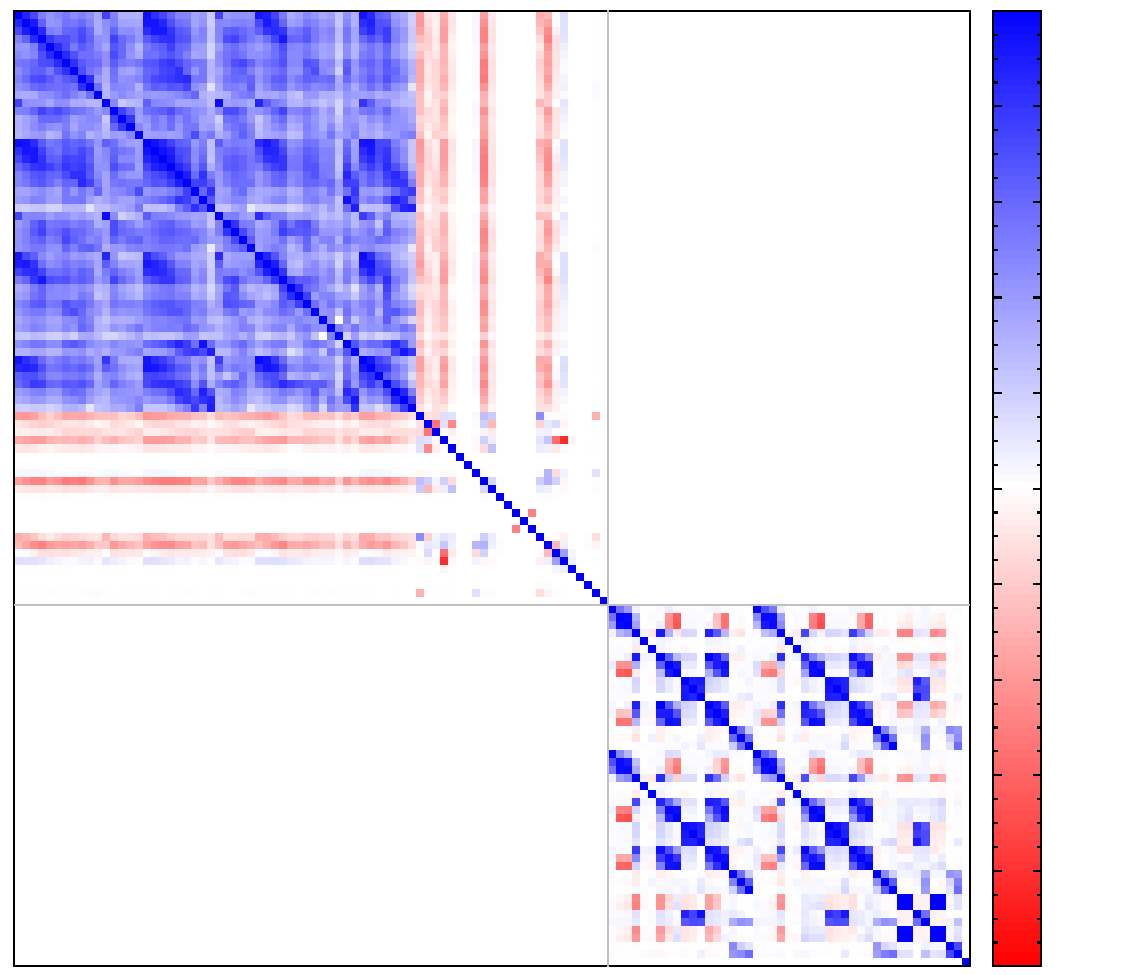
\includegraphics{matrixplot}}%
    \gplfronttext
  \end{picture}%
\endgroup
}
	\caption[Correlation matrix of the T2K systematic model]%
		{Correlation matrix of the T2K systematic model.
		The two main blocks correspond to respectively the BANFF errors and the far detector %
		Final State interaction errors.}
	\label{fig:correlation}
\end{figure}

The relative $f_j^n$ terms for the beam errors are loaded from four different ROOT files, %
one for each event sample (see below).
They are saved as \texttt{TH1D} objects and are identified by numbers, instead of names.
The correlation matrix is stored under a separate ROOT file as a \texttt{TMatrix} object.
The correlation matrix between the beam systematics is shown as a 2D colour map on \reffig{fig:correlation}, %
from which the three main typologies of uncertainties\,---\,flux, cross-section, and far detector\,---\,%
are easily recognised.
The SK and FSI systematics are visibly uncorrelated with the BANFF ones.


The beam sample is created using a far detector flux prediction, differently from the atmospheric sample which is created with MC files.
Fully-contained candidate events in the fiducial volume are grouped %
as appearance signals, i.e.\ $\nu_\mu\to\nu_e$ and $\cj{\nu}_\mu\to\cj{\nu}_e$, %
and background events from disappearance channels.
Signal and background distributions in true energy (98 bins) undergo event selection criteria %
to obtain the distributions in reconstructed energy (87 bins) for the four event samples: %
\begin{multicols}{2}
	\begin{itemize}
		\item one ring $e$-like in $\nu$-mode; %
		\item one ring $\mu$-like in $\nu$-mode; %
		\item one ring $e$-like in $\cj{\nu}$-mode; %
		\item one ring $\mu$-like in $\cj{\nu}$-mode.
	\end{itemize}
\end{multicols}
A set of 2D smearing matrices, produced by the T2K fitting framework VALOR~\cite{VALOR}, %
simulates and replaces the correct event selection process, including tuning of the flux with near detector constraints.
These smearing matrices are provided for all samples, acting on signal (CCQE and CCnQE) %
and background (CCQE, CCnQE, and NC) distributions, and are used to convert the prediction from true energy to reconstructed energy.
They are engineered such that the near detector prediction in true energy bins is already included in the matrices %
and the far detector prediction is just a row-wise sum of these matrices
\begin{equation}
	\phi(E_\text{reco}) = \sum_j M\ \vec{1}(E_\text{true})
\end{equation}
and oscillation probability is simply applied in the following way
\begin{equation}
	\phi(E_\text{reco}) = \sum_j M\ \vec{P}_{\nu_\alpha \to \nu_\beta}(E_\text{true})\ ,
\end{equation}
where the index $j$ runs over the interaction mode.
The one ring $e$-like with one electron decay sample, included in T2K analyses, is not considered in this study.


The card file for the beam sample class looks like this
\begin{lstlisting}[language=bash]
    # scale statistics, 1.00 = 100% of data
    stats	1.00
    
    # density profile for beamline
    density_profile	"data/DensityProfileTochibora.dat"
    
    
    # specify which samples to fit
    # if commented, all of them are used
    #sample	"E_FHC", "E_RHC", "M_FHC", "M_RHC" # example
    
    
    #energy scale error for E-like or M-like
    scale_error	0.024	# if just one
    
    #scale_error_E	0.024	# if independent
    #scale_error_M	0.024
    
    #restrict systematics
    syst_first	0
    syst_last	110
    # systematics to skip, as a number
    skip		55, 56, 73
    
    #systematic information
    corr_file	"errorstudy/one/systematics/matrix.root"
    corr_name	"correlation"
    
    systematic_E_FHC "errorstudy/one/systematics/E_FHC.root"
    systematic_E_RHC "errorstudy/one/systematics/E_RHC.root"
    systematic_M_FHC "errorstudy/one/systematics/M_FHC.root"
    systematic_M_RHC "errorstudy/one/systematics/M_RHC.root"
    
    reco_input	"/somewhere/in/reconstruction_atmo"
\end{lstlisting}


\section{Chi squared class}
\label{sec:x2}

The chi squared class is used to combine different samples, which inherited from the sample class, and %
computed the $\chi^2$ between two different sets of oscillation parameters.

The \emph{true} combination of oscillation parameters is typically fixed and used to build the %
``observed'' event samples.
The \emph{fit} combination is changed at each iteration to created the ``expected`` event samples %
and the $\chi^2$ is computed by comparing these two different predictions.
By scanning through the oscillation parameter space, it is possible to study the dependence of the $\chi^2$ %
with respect to oscillation parameters and so determine the sensitivity of the experiment of reject null hypotheses.
For example, the exclusion regions for CP conservation is defined by changing the \emph{true} value of the CP phase %
and by comparing the $\chi^2$ at any value of $\delta_\text{CP}$ with the $\chi^2$ computed at %
the null hypothesis, i.e.\ CP conservation or $\delta_\text{CP} = 0, \pm\pi$.
The exclusion sensitivity as a function of \emph{true} $\delta_\text{CP}$ %
is quantified by %
\begin{equation}
	\sigma = \sqrt{\min_{\delta_\text{CP} = 0,\pm\pi}\! \chi^2\  -\,\chi^2_\text{\emph{true}}}\ ,
\end{equation}
where $\chi^2_\text{\emph{true}}$ is evaluated at the \emph{true} point and matches the best fit value.

A ChiSquared object is created with the constructors
\begin{lstlisting}[language=C++]
(1) ChiSquared(CardDealer *card);
(2) ChiSquared(std::string card);
\end{lstlisting}
where the card contains control parameters for the minimisation and Levenberg-Marquartd algorithm.
The same object should be used to create locally the sample objects with the following templated function
\begin{lstlisting}[language=C++]
    template <class S> void Add(std::string card);
\end{lstlisting}
where the class \texttt{S} inherits from the Sample base class.
The input card file is the respective sample configuration file.
After loading/creating the adequate number of samples, the method
\begin{lstlisting}[language=C++]
    void Combine();
\end{lstlisting}
should be called to initialise the sample and the ChiSquared classes.
The event samples and systematic errors are combined into local objects to facilitate the minimisation algorithm.
The ChiSquared class is friend to Sample-derived classes and so special methods to access member variables are not needed.

Let us define the likelihood
\begin{equation}
	\mathfrak{L}(E_n, O_n) = \prod_n \frac{e^{-E_n} E_n^{O_n}}{O_n!}\ ,
\end{equation}
where $O_n$ and $E_n$ are respectively the number of observed and expected events in the $n$-th bin, %
which are built using a specific combination of oscillation parameters and a given mass hierarchy $H$
\begin{equation}
	\Theta^H \equiv (\Delta m^2{21}, |\Delta m^2_{32}|, \sin^2\theta_{12}, \sin^2 2\theta_{13}, \sin^2 \theta_{23}, \delta_\text{CP})\ .
\end{equation}
The expected events are defined by a prediction at the far detector weighted by the oscillation probabilities %
for parameters $\Theta$, and since there is no real data yet the ``observed'' events are also given by %
a prediction weighted with the \emph{true} oscillation point, $\Theta^H_\text{true}$.
%and the product runs over the total number of bins.
The $\chi^2$ is hence the following log-likelihood ratio
\begin{equation}
	\label{eq:log_ratio}
	\chi^2(\Theta^H) = -2 \log \qty[\frac{\mathfrak{L}(E_n, O_n)}{\mathfrak{L}(O_n, O_n)}] =
		2 \sum_n \qty[E_n - O_n + O_n \log \qty(\frac{O_n}{E_n})]\ ,
\end{equation}
which is modified according to the ``pull approach'' $\chi^2$~\cite{Fogli:2002pt}: %
the parameters $\bs{\varepsilon} = \{\varepsilon_j\}$ are introduced %
to account for systematic uncertainties by replacing
\begin{equation}
	\label{eq:pull}
	E_n\ \longrightarrow\ E_n\,\prod_j \qty(1 + f_j^n \varepsilon_j)\ ,
\end{equation}
where the index $j$ runs over the systematic parameters.
A penalty term that includes variances and covariances of such parameters is added to the likelihood, %
using the inverse of the correlation matrix of the systematic errors, $\rho^{-1}$.
The effect of the systematic uncertainties on the event distributions is embedded in the $f_j^n$ parameters, %
defined as the fractional change induced on the $n$-th bin by a 1\,$\sigma$ variation of the $j$-th systematic.
The amount of change is therefore parameterised by the $\varepsilon_j$ variables in units of the uncertainty $\sigma_j$.
However, being $\rho$ the correlation matrix, the $\varepsilon_j$ are promoted to embody the systematic uncertainties.
Energy scale shifting parameters are treated differently because they act on the binning rather than on the %
bin contents.
Its effect on the $n$-th bin of the expected events is analytically represented as
\begin{equation}
	E_n' = \sum_m \frac{E_m\,\textstyle\prod_i(1 + \varepsilon_i f^i_m)}%
	{4\ (1+\sk \sigma)\, \Delta b_m} \beta_{n, m}(1+\sk \sigma)\ ,
\end{equation}
where
\begin{align}
	\beta_{n, m}(x) &= (1 + s_\beta) (\Delta b_n + x\, \Delta b_m - \abs{b_n - x\, b_m} - \abs{b_{n+1} - x\, b_{m+1}} ) \notag \\
	s_\beta &= \text{sign} (\Delta b_n + x\, \Delta b_m - \abs{b_n - x\, b_m} - \abs{b_{n+1} - x\, b_{m+1}} )\ .
\end{align}
is a ``mask'' function that quantifies the overlap between shifted and nonshifted bins.
The amount of shift is $1+\sk \sigma$, where $\sigma$ is the scale error and $\sk$ the error parameter.
The term $1 + s_\beta$  makes $\beta_{n,m}(x)$ strictly nonnegative, meaning it is positive or zero, %
and its derivative
\begin{equation}
	\pdv{\beta_{n,m}(1+\sk\sigma)}{\sk} = 
	\sigma\ \pdv{\beta_{n,m}}{x}\eval_{x=1+\sk\sigma} = \sigma\ (1 + s_\beta)
	\qty(\Delta b_m + \frac{b_n - b_m}{|b_n - b_m|} b_m + \frac{b_{n+1} - b_{m+1}}{|b_{n+1} - b_{m+1}|} b_{m+1})
\end{equation}
does not depend on the shift amount $x$.
With all these adjustments included, the total $\chi^2$ reads
\begin{equation}
	\chi^2_\text{tot}(\Theta^H) = 2 \sum_n \qty[ E_n' - O_n - O_n \log \frac{E_n'}{O_n} ]
	+ \sum_{kj} \varepsilon_k \rho^{-1}_{kj} \varepsilon_j\ .
\end{equation}

The $\chi^2$ can be calculated having the observed and expected spectra and the error parameters.
These three objects are represented by \texttt{Eigen::VectorXd} objects and are used with the following public functions
\begin{lstlisting}[language=C++]
(1) double X2(const Eigen::VectorXd &On,
              const Eigen::VectorXd &En,
              const Eigen::VectorXd &epsil);
(2) double SysX2(const Eigen::VectorXd &epsil);
(3) double ObsX2(const Eigen::VectorXd &On,
                 const Eigen::VectorXd &En,
                 const Eigen::VectorXd &epsil);
(4) Eigen::ArrayXd ObsX2n(const Eigen::VectorXd &On,
                          const Eigen::VectorXd &En,
                          const Eigen::VectorXd &epsil);
    
(5) double RawX2(const Eigen::VectorXd &On,
                 const Eigen::VectorXd &En);
(6) Eigen::ArrayXd RawX2n(const Eigen::VectorXd &On,
                          const Eigen::VectorXd &En);
\end{lstlisting}
The function \texttt{(1)} calls \texttt{(2)} and \texttt{(3)} which respectively %
compute the systematic and statistical contribution of the $\chi^2$.
The function \texttt{ObsXn} \texttt{(4)} returns the $\chi^2$ bin-by-bin as an array, %
such that the sum of this array bin contents equals to the output of \texttt{ObsX2)}.
The last two function \texttt{(5)} and \texttt{(6)} compute the $\chi^2$ without the %
contribution of systematic parameters and are useful for debugging purposes.

The $\chi^2$ needs to be profiled with respect to the systematic parameters~$\bs{\varepsilon}$:
\begin{equation}
	\label{eq:chi2_min}
	\chi^2(\Theta^H) = \min_{\bs{\varepsilon}}\, \qty\Big[\,\chi^2(\Theta^H;\bs{\varepsilon})\,]\ .
\end{equation}
Fixing the combination $\Theta^H$ and dropping it from the notation, %
the minimisation of the $\chi^2$ leads to the following set of $j$ nonlinear equations %,
\begin{equation}
	\pdv{\chi^2}{\varepsilon_j} (\bs{\varepsilon}) = 0\ 
\end{equation}
which is solved iteratively with the Levenberg-Marquardt (LM) method~\cite{Levenberg_1944, Marquardt_1963}.
The equations to solve at each step is
\begin{equation}
	\qty[\pdv{\chi^2(\bs{\varepsilon}^{(n)})}{\varepsilon_k}{\varepsilon_j} %
	+ \lambda \max \qty(\text{diag} \pdv{\chi^2(\bs{\varepsilon}^{(n)})}{\varepsilon_k}{\varepsilon_j}) \mathbb{1}]
	\cdot \qty(\varepsilon_j^{(n+1)} - \varepsilon_j^{(n)}) = %
	-\pdv{\chi^2(\bs{\varepsilon}^{(n)})}{\varepsilon_k}\ .
\end{equation}
The parameter $\lambda$ is chosen dynamically: if the cost function $\chi^2$ decreases %
after an iteration step, then $\lambda$ is reduced; otherwise $\lambda$ is increased and the step recomputed.
In the limit $\lambda \to 0$, the algorithm approximates the Gauss-Newton's method and its fast convergence.
When $\lambda$ is large, the linear system resembles a gradient descent with small steps of the order of $\lambda^{-1}$, %
but with a more stable convergence.
A ``delayed-gratification scheme'' is adopted for $\lambda$~\cite{Transtrum2012}, using an initial value of $\lambda^{(0)} = 1$ and finding %
an optimal increment and decrement of respectively $\lambda^{(n+1)} = 5\,\lambda^{(n)}$ and $\lambda^{(n+1)} = \lambda^{(n)} / 10$.
The Jacobian of the $\chi^2$ is 
\begin{equation}
	\pdv{\chi^2}{\varepsilon_k} =
	2\sum_n \qty[\pdv{E_n'}{\varepsilon_k}\qty(1 - \frac{O_n}{E_n'})]
	+ 2\sum_j \rho^{-1}_{kj} \varepsilon_j
\end{equation}
whereas the Hessian is
\begin{equation}
	\pdv{\chi^2}{\varepsilon_k}{\varepsilon_j} =
	2\sum_n \qty[\pdv{E_n'}{\varepsilon_k}{\varepsilon_j} \qty(1 - \frac{O_n}{E_n'})
	+ \frac{O_n}{E_n'^2} \pdv{E_n'}{\varepsilon_k} \pdv{E_n'}{\varepsilon_j}]
	+ 2 \rho^{-1}_{kj}
\end{equation}
and they are both computed simultaneously by 
\begin{lstlisting}[language=C++]
    void JacobianHessian(Eigen::VectorXd &jac, Eigen::MatrixXd &hes,
			 const Eigen::VectorXd &On, const Eigen::VectorXd &En,
			 const Eigen::VectorXd &epsil);
\end{lstlisting}
which implements the following derivative terms
\begin{align}
	\pdv{E_n'}{\varepsilon_k} &= \sum_m \frac{E_m\,\textstyle\prod_i(1 + \varepsilon_i f^i_m)}%
		{4\ (1+\sk \sigma)\, \Delta b_m} \beta_{n, m}(1+\sk \sigma) \frac{f_m^k}{1+\varepsilon_k f^k_m} \\
	\pdv{E_n'}{\sk} &= \sum_m \frac{E_m\,\textstyle\prod_i(1 + \varepsilon_i f^i_m)}%
		{4\, \Delta b_m} \frac{\sigma}{1 + \sk \sigma} \qty(\pdv{\beta_{n, m}}{x} -\frac{\beta_{n,m}(1+\sk\sigma)}{1+\sk \sigma} ) \\
	\pdv{E_n'}{\varepsilon_k}{\varepsilon_j} &= \sum_m \frac{E_m\,\textstyle\prod_i(1 + \varepsilon_i f^i_m)}%
		{4\ (1+\sk \sigma)\, \Delta b_m} \beta_{n, m}(1+\sk \sigma)\ \frac{f_m^k\ f_m^j}{(1+\varepsilon_k f^k_m)(1+\varepsilon_j f^j_m)} \\
	\pdv{E_n'}{\varepsilon_k}{\sk} &= \sum_m \frac{E_m\,\textstyle\prod_i(1 + \varepsilon_i f^i_m)}%
		{4\, \Delta b_m} \frac{\sigma}{1 + \sk \sigma} \qty(\pdv{\beta_{n, m}}{x} -\frac{\beta_{n,m}(1+\sk\sigma)}{1+\sk \sigma} )
		\,\frac{f_m^k}{1+\varepsilon_k f^k_m} \\
	\pdv[2]{E_n'}{\sk} &= \sum_m \frac{E_m\,\textstyle\prod_i(1 + \varepsilon_i f^i_m)}%
		{2\, \Delta b_m} \frac{\sigma^2}{(1 + \sk \sigma)^2} \qty(\frac{\beta_{n,m}(1+\sk\sigma)}{1+\sk \sigma} - \pdv{\beta_{n, m}}{x})
\end{align}

Energy scaling is a slow operation because it requires a summation over all the samples for each bin of the event sample.
During the computation of the Jacobian and Hessian this is needed multiple times and the dimension of these two matricial objects %
is substantial.
Various preventive measures are taken together with heavy optimisation of the code.
The scaling of the bin axes is precomputed for each sample (beam or atmospheric) and stored in each of its variation (see derivatives above) %
in the following fixed vectors of dimension as number of event bins
\begin{align*}
	\xi^n_m &= \frac{1}{4\ (1+\sk \sigma)\, \Delta b_m}  \ 
	\beta_{n, m}(1+\sk \sigma) \\
	\pdv{\xi_m}{\sk} &= \frac{1}{4\ (1+\sk \sigma)\, \Delta b_m}\ 
	\sigma\ \qty(\pdv{\beta_{n, m}}{x} - \frac{\beta_{n,m}(1+\sk\sigma)}{1+\sk \sigma}) \\
	\pdv[2]{\xi_m}{\sk} &= \frac{1}{4\ (1+\sk \sigma)\, \Delta b_m}\ 
	\frac{2\sigma^2}{(1+\sk \sigma)}\,\qty(\frac{\beta_{n,m}(1+\sk\sigma)}{1+\sk \sigma} - \pdv{\beta_{n, m}}{x}) \\
\end{align*}
They only depend just on the energy scaling and its error.
If the event samples are also expressed as vectors $\tilde{E}_m = E_m \prod_j (1+\varepsilon_j f^j_m)$, %
then the ``shifted'' content of the $n$-th bin can be expressed as a coefficient-wise (Hadamard) product, e.g.\ 
\begin{equation}
	E_n' = \tilde{E}^T\ \xi^n = \sum_m \tilde{E}_m\, \xi^n_m
\end{equation}
Similarly, the derivative with respect to a non-energy scale parameter can be vectorised as
\begin{equation}
	\pdv{\tilde{E}_n}{\varepsilon_k} = \tilde{E}_n \frac{f_k^n}{1 + \varepsilon_k f_n^k} =
	E_n \frac{f_k^n}{1 + \varepsilon_k f_n^k}{\textstyle\prod_i} (1 + \varepsilon_i f_n^i) 
\end{equation}
and so derivatives and second derivatives can be expressed as coefficient-wise products between %
the event samples, the derivative vectors, and the energy scale vectors (see previous slide).
Defining
\[
	\gamma^k_m = \frac{f_m^k}{1+\varepsilon_k f_m^k}
\]
we have for example
\begin{align}
	\pdv{E_n'}{\varepsilon_k} &= \tilde{E}^T\ \text{diag}(\gamma^k)\ \xi^n %
	= \sum_m \tilde{E}_m\, \gamma^k_m\, \xi^n_m \\
	\pdv{E_n'}{\varepsilon_k}{\varepsilon_j} &=
	\tilde{E}^T\ \text{diag}(\gamma^k)\, \text{diag}(\gamma^j)\ \xi^n
	= \sum_m \tilde{E}_m\, \gamma^k_m\, \gamma^j_m\, \xi^n_m \\
\end{align}
Thanks to the Eigen library, the Hadamard products can be compiled as vectorised instruction for the CPU, %
speeding up the computation.

The LM algorithm is implemented in 
\begin{lstlisting}[language=C++]
    unsigned int MinimumX2(const Eigen::VectorXd &On,
			   const Eigen::VectorXd &En,
			   Eigen::VectorXd &epsil, double &x2);
\end{lstlisting}
which finds the combination of $\bs{\varepsilon}$ which minimised the $\chi^2$.
The function should be called within 
\begin{lstlisting}[language=C++]
    Eigen::VectorXd FitX2(const Eigen::VectorXd &On,
		          const Eigen::VectorXd &En);
\end{lstlisting}
which handles the error code returns of \texttt{MinimumX2}.
The method \texttt{FitX2} makes sure the minimisation process is proceeding in the right direction %
as the LM can sometimes not converge, go out of the boundaries, or stop not at the absolute minimum.
Thanks to the error codes, \texttt{FitX2} might decide to move the solution $\bs{\varepsilon}$ to %
a different point to facilitate the LM algorithm.
This is done with random trials looking for a point with a smaller $\chi^2$ in the direction of the best point.
The maximum number of random trials is set in the card file with key \texttt{max\_random\_trials}.
The process is repeated until either the LM converges to sufficient error \texttt{fit\_error} or %
the maximum number of iteration \texttt{max\_iteration} is reached.
The LM algorithm does not have a maximum number of iteration and it quits when the step taken is smaller than \texttt{fit\_error}.
Note that the overall minimisation process always starts at $\bs{\varepsilon} = 0$.


\bibliography{biblio.bib}

\end{document}

